\documentclass[11pt]{article}

% ---------- Packages (per course conventions) ----------
\usepackage[margin=1in]{geometry}
\usepackage{graphicx}
\usepackage{float}
\usepackage{booktabs}
\usepackage{siunitx}
\usepackage{amsmath}
\usepackage{amssymb}
\usepackage{tikz}
\usetikzlibrary{arrows.meta,calc,angles,quotes,decorations.pathmorphing}
\usepackage{tcolorbox}
\usepackage{enumitem}
\usepackage{xcolor}
\usepackage{hyperref}
\hypersetup{colorlinks=true, linkcolor=black, urlcolor=blue}

\setlength{\parindent}{0pt}
\setlength{\parskip}{\baselineskip}

% =========================================================
% EDIT THESE FOR EACH NEW ASSIGNMENT
% =========================================================
\newcommand{\assignmentNumber}{3}
\newcommand{\assignedDate}{25 Sept 2026}
\newcommand{\dueDate}{2 Oct 2026 (11:59pm, Moodle)}
\newcommand{\numProblems}{8}

% ---------- unit shorthands ----------
\newcommand{\lb}{\,\mathrm{lb}}
\newcommand{\N}{\,\mathrm{N}}
\newcommand{\kN}{\,\mathrm{kN}}
\newcommand{\m}{\,\mathrm{m}}
\newcommand{\kNm}{\,\mathrm{kN{\cdot}m}}
\newcommand{\ft}{\,\mathrm{ft}}
\newcommand{\kg}{\,\mathrm{kg}}

% ---------- Boxed-answer helper ----------
\newtcolorbox{finalanswer}{
    colback=white, colframe=black, boxrule=1pt,
    title=Answer, fonttitle=\bfseries, coltitle=black,
    colbacktitle=white
}

% ---------- Force-arrow style for sketches ----------
\tikzset{
  frc/.style={-{Stealth[length=2.6mm]}, very thick, red!70!black},
  dimn/.style={{Stealth[length=1.8mm]}-{Stealth[length=1.8mm]}, thin},
  ax/.style={-{Stealth[length=2mm]}, thin, gray!70!black},
  mem/.style={line width=2.2pt, blue!50!black!70},
}

% ---------- Reusable problem scaffold ----------
% \problempage{num}{summary}{sketch code (tikzpicture)}{equations & solution}{answer}
\newcommand{\problempage}[5]{%
    \clearpage
    \section*{Problem #1}

    \textbf{Given / Find:} #2

    \textbf{Sketch:}

    \begin{center}
    #3
    \end{center}

    \textbf{Equations \& Solution:}

    #4

    \begin{finalanswer}
    #5
    \end{finalanswer}
}

\begin{document}

% =========================================================
% COVERSHEET
% =========================================================
\begin{titlepage}
    \centering
    \vspace*{2cm}
    {\LARGE \bfseries ENGR 225: Mechanics 1} \\[0.3cm]
    {\Large Homework Coversheet} \\[0.3cm]
    {\large Assoc.\ Prof.\ Clayton Byers} \\[2cm]

    \begin{flushleft}
        \Large
        \textbf{NAME:} \underline{\hspace{0.5cm}Sean Balbale\hspace{6.5cm}} \\[1cm]
        \textbf{DATE:} \underline{\hspace{0.5cm}\hspace{9cm}} \\[1cm]
        \textbf{ASSIGNMENT:} \underline{\hspace{0.5cm}Homework 3\hspace{5.5cm}} \\[2cm]
    \end{flushleft}

    \large
    \textbf{Level of involvement of AI, LLMs, or related tools in the completion of this assignment:}

    \vspace{1cm}

    \begin{flushleft}
        \Large
        $\square$ \quad None \\[0.7cm]
        $\blacksquare$ \quad Minor \\[0.7cm]
        $\square$ \quad Major \\[0.7cm]
        $\square$ \quad Extensive \\[1.5cm]
    \end{flushleft}

    \normalsize
    \textit{Mark the box that applies (e.g., replace $\square$ with $\blacksquare$, or type an X beside it, before compiling/printing). Your disclosure does not affect your grade -- it keeps you accountable for the work you are doing.}

\end{titlepage}

% % =========================================================
% % HOMEWORK HEADER
% % =========================================================
% \section*{ENGR 225 -- Homework \assignmentNumber}
% \textbf{Assigned:} \assignedDate \hfill \textbf{Due:} \dueDate

% \vspace{0.3cm}
% \textit{Formatting per course guidelines: each problem on its own page, with problem summary, labeled sketch, governing equations, units carried throughout, results to 3 significant figures, and a clearly boxed final answer.}

% =========================================================
% PROBLEM 1
% =========================================================
\problempage{1}{
A seat-restraint pressure on the head varies parabolically, $w(x)=12(1+2x^2)$ lb/ft, for $0\le x\le 0.5$ ft measured from A (12 lb/ft at A, 18 lb/ft at B). \textbf{Find} the equivalent resultant force $F$ and its location $\bar{x}$ from A.
}{
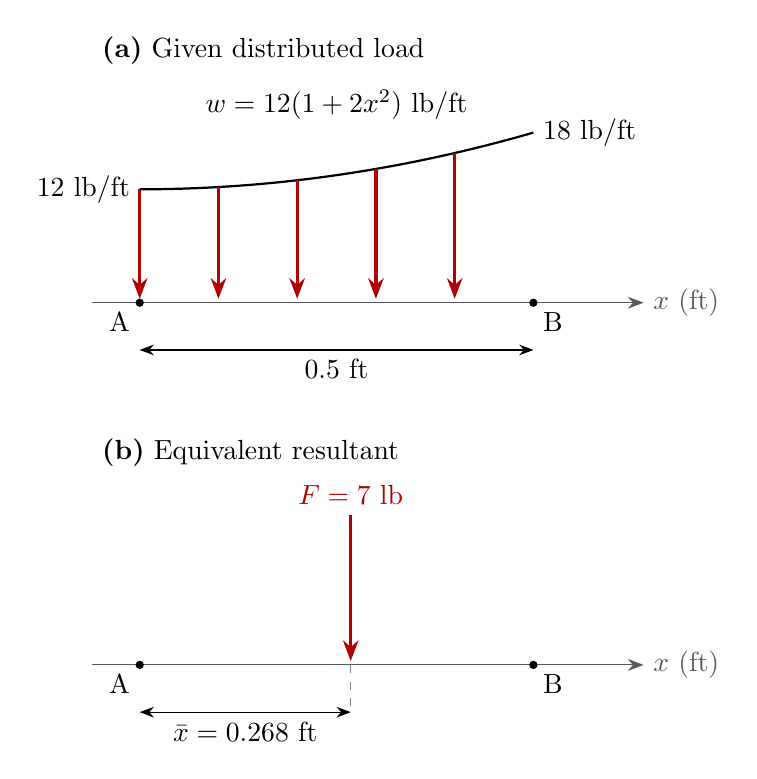
\begin{tikzpicture}[scale=1]
  % --- (a) given loading ---
  \draw[ax] (-0.6,0) -- (6.4,0) node[right] {$x$ (ft)};
  \draw[thick] plot[domain=0:0.5,samples=40] ({10*\x},{0.12*12*(1+2*\x*\x)});
  \foreach \xx in {0,0.1,...,0.5}{
    \draw[frc] ({10*\xx},{0.12*12*(1+2*\xx*\xx)}) -- ({10*\xx},0.05);
  }
  \fill (0,0) circle (1.5pt) node[below left] {A};
  \fill (5,0) circle (1.5pt) node[below right] {B};
  \node[left] at (0,1.44) {12 lb/ft};
  \node[right] at (5,2.16) {18 lb/ft};
  \node[above] at (2.5,2.2) {$w=12(1+2x^2)$ lb/ft};
  \draw[dimn] (0,-0.6) -- (5,-0.6) node[midway,below] {0.5 ft};
  \node[anchor=west] at (-0.6,3.2) {\textbf{(a)} Given distributed load};
  % --- (b) equivalent ---
  \begin{scope}[yshift=-4.6cm]
    \draw[ax] (-0.6,0) -- (6.4,0) node[right] {$x$ (ft)};
    \fill (0,0) circle (1.5pt) node[below left] {A};
    \fill (5,0) circle (1.5pt) node[below right] {B};
    \draw[frc] (2.68,1.9) -- (2.68,0.05) node[pos=0,above] {$F=7$ lb};
    \draw[dimn] (0,-0.6) -- (2.68,-0.6) node[midway,below] {$\bar{x}=0.268$ ft};
    \draw[dashed,gray] (2.68,0) -- (2.68,-0.6);
    \node[anchor=west] at (-0.6,2.7) {\textbf{(b)} Equivalent resultant};
  \end{scope}
\end{tikzpicture}
}{
The resultant force equals the area under the load curve, and it acts at the centroid of that area:
\begin{align*}
F &= \int_0^{0.5} w\,dx = \int_0^{0.5} 12\,(1+2x^2)\,dx
   = 12\left[x+\tfrac{2}{3}x^3\right]_0^{0.5\ft}\ \tfrac{\mathrm{lb}}{\mathrm{ft}}\\
  &= 12\left(0.5+\tfrac{2}{3}(0.125)\right)\lb = 12(0.5833)\lb = 7.00\lb\\[4pt]
\bar{x} &= \frac{\int_0^{0.5} x\,w\,dx}{\int_0^{0.5} w\,dx}
  = \frac{12\left[\tfrac{x^2}{2}+\tfrac{x^4}{2}\right]_0^{0.5}\ \mathrm{lb}}{7.00\lb}
  = \frac{12\,(0.125+0.03125)\ \mathrm{lb{\cdot}ft}}{7.00\lb}
  = \frac{1.875\ \mathrm{lb{\cdot}ft}}{7.00\lb} = 0.268\ft
\end{align*}
Check: $\bar{x}=0.268$ ft is slightly greater than $0.25$ ft (the midpoint) because the load is heavier at B.
}{
$F = 7.00\lb$ (in the direction of the pressure), acting at $\bar{x} = 0.268\ft$ from A.
}

% =========================================================
% PROBLEM 2
% =========================================================
\problempage{2}{
A 12 m beam carries a triangular load (peak 6 kN/m at $x=7.5$ m, zero at both ends), a 15 kN point load at the right end ($x=12$ m), and a 500 kN$\cdot$m clockwise couple at O. \textbf{Find} the equivalent single force $F_R$ and couple moment $M_R$ acting at O. (Counterclockwise moments are taken positive.)
}{
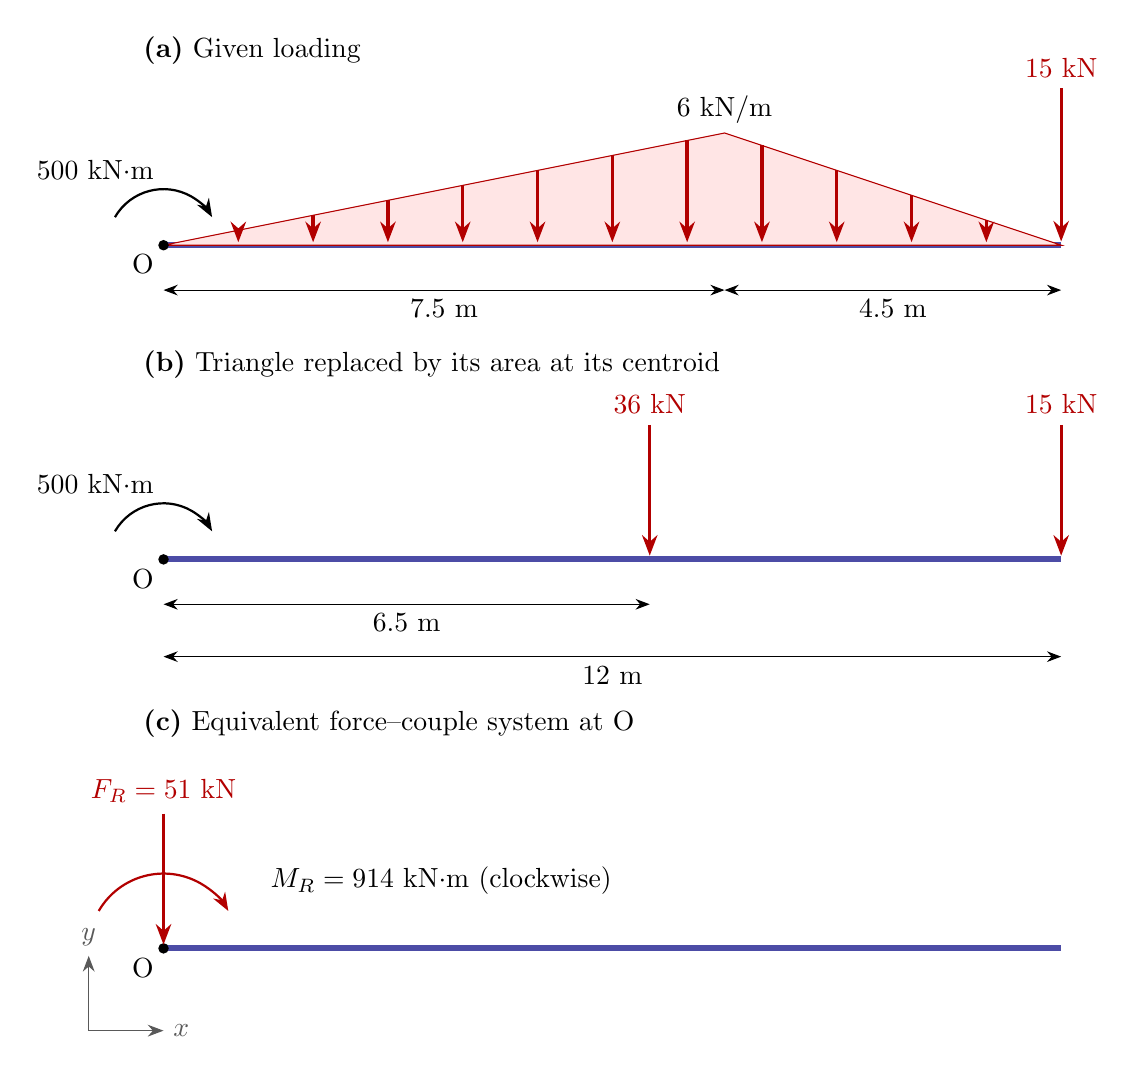
\begin{tikzpicture}[scale=0.95]
  % --- (a) given ---
  \draw[mem] (0,0) -- (12,0);
  \draw[fill=red!10,draw=red!70!black] (0,0) -- (7.5,1.5) -- (12,0) -- cycle;
  \foreach \xx in {1,2,...,11}{
    \pgfmathsetmacro{\h}{ifthenelse(\xx<=7.5, 1.5*\xx/7.5, 1.5*(12-\xx)/4.5)}
    \draw[frc] (\xx,\h) -- (\xx,0.04);
  }
  \draw[frc] (12,2.1) -- (12,0.05) node[pos=0,above] {15 kN};
  \node[above] at (7.5,1.5) {6 kN/m};
  \draw[thick,-{Stealth}] (150:0.75) arc (150:30:0.75);
  \node[above left] at (0,0.75) {500 kN$\cdot$m};
  \fill (0,0) circle (2pt) node[below left] {O};
  \draw[dimn] (0,-0.6) -- (7.5,-0.6) node[midway,below] {7.5 m};
  \draw[dimn] (7.5,-0.6) -- (12,-0.6) node[midway,below] {4.5 m};
  \node[anchor=west] at (-0.4,2.6) {\textbf{(a)} Given loading};

  % --- (b) concentrated loads ---
  \begin{scope}[yshift=-4.2cm]
    \draw[mem] (0,0) -- (12,0);
    \draw[frc] (6.5,1.8) -- (6.5,0.05) node[pos=0,above] {36 kN};
    \draw[frc] (12,1.8) -- (12,0.05) node[pos=0,above] {15 kN};
    \draw[thick,-{Stealth}] (150:0.75) arc (150:30:0.75);
    \node[above left] at (0,0.75) {500 kN$\cdot$m};
    \fill (0,0) circle (2pt) node[below left] {O};
    \draw[dimn] (0,-0.6) -- (6.5,-0.6) node[midway,below] {6.5 m};
    \draw[dimn] (0,-1.3) -- (12,-1.3) node[midway,below] {12 m};
    \node[anchor=west] at (-0.4,2.6) {\textbf{(b)} Triangle replaced by its area at its centroid};
  \end{scope}

  % --- (c) at O ---
  \begin{scope}[yshift=-9.4cm]
    \draw[mem] (0,0) -- (12,0);
    \fill (0,0) circle (2pt);
    \draw[frc] (0,1.8) -- (0,0.05) node[pos=0,above] {$F_R=51$ kN};
    \draw[thick,-{Stealth},red!70!black] (150:1) arc (150:30:1);
    \node[right] at (1.3,0.9) {$M_R=914$ kN$\cdot$m (clockwise)};
    \node[below left] at (0,0) {O};
    \draw[ax] (-1,-1.1) -- (0,-1.1) node[right] {$x$};
    \draw[ax] (-1,-1.1) -- (-1,-0.1) node[above] {$y$};
    \node[anchor=west] at (-0.4,3.0) {\textbf{(c)} Equivalent force--couple system at O};
  \end{scope}
\end{tikzpicture}
}{
\textbf{Step 1 -- replace the triangular load by its area, placed at its centroid.} The triangle has base $12$ m and height $6$ kN/m; its centroid lies one-third of the sum of the vertex positions ($0$, $7.5$, $12$ m) from O:
\begin{align*}
W_\triangle &= \tfrac12(12\m)(6\ \mathrm{kN/m}) = 36.0\kN, &
\bar{x}_\triangle &= \frac{0+7.5+12}{3}\m = 6.5\m
\end{align*}
\textbf{Step 2 -- resultant force} (upward positive):
\[
\sum F_y:\quad F_R = -36.0\kN - 15.0\kN = -51.0\kN 
\]
\textbf{Step 3 -- resultant moment about O}:
\begin{align*}
M_R &= \sum M_O = -500\kNm - (36.0\kN)(6.5\m) - (15.0\kN)(12\m)\\
    &= -500\kNm - 234\kNm - 180\kNm = -914\kNm
\end{align*}
The negative signs mean the resultant force points downward and the couple is clockwise.
}{
$F_R = -51.0\kN$ (51.0 kN downward) and $M_R = -914\kNm$ (914 kN$\cdot$m clockwise), both acting at O.
}

% =========================================================
% PROBLEM 3
% =========================================================
\problempage{3}{
Frame ABC carries a 3 kN/m load downward along the 3 m horizontal member AB and a 2 kN/m load acting leftward along the 4 m vertical member BC. \textbf{Find} the single equivalent resultant force $\vec{R}$ and the distance $d$ from A to where its line of action crosses the horizontal line through AB.
}{
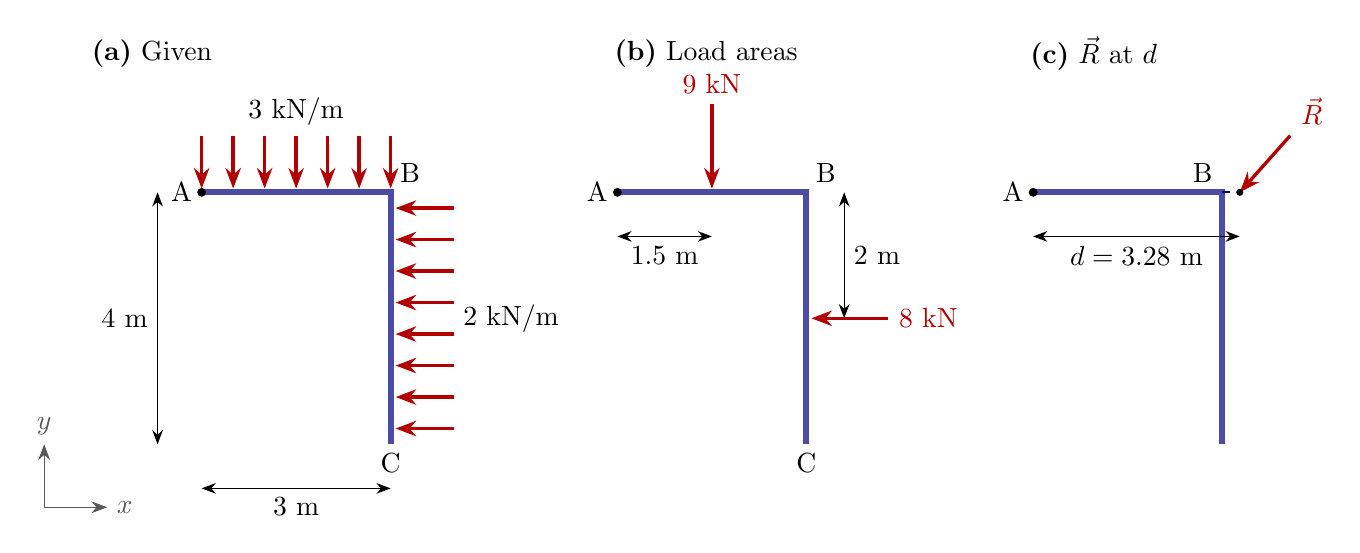
\begin{tikzpicture}[scale=0.8]
  % --- (a) given ---
  \draw[mem] (0,0) -- (3,0) -- (3,-4);
  \fill (0,0) circle (2pt) node[left] {A};
  \node[above right] at (3,0) {B};
  \node[below] at (3,-4) {C};
  \foreach \xx in {0,0.5,...,3}{ \draw[frc] (\xx,0.9) -- (\xx,0.06); }
  \node[above] at (1.5,0.9) {3 kN/m};
  \foreach \yy in {-0.25,-0.75,...,-3.75}{ \draw[frc] (4,\yy) -- (3.08,\yy); }
  \node[right] at (4,-2) {2 kN/m};
  \draw[dimn] (0,-4.7) -- (3,-4.7) node[midway,below] {3 m};
  \draw[dimn] (-0.7,0) -- (-0.7,-4) node[midway,left] {4 m};
  \draw[ax] (-2.5,-5) -- (-1.5,-5) node[right] {$x$};
  \draw[ax] (-2.5,-5) -- (-2.5,-4) node[above] {$y$};
  \node[anchor=west] at (-1.9,2.2) {\textbf{(a)} Given};

  % --- (b) equivalent point loads ---
  \begin{scope}[xshift=6.6cm]
    \draw[mem] (0,0) -- (3,0) -- (3,-4);
    \fill (0,0) circle (2pt) node[left] {A};
    \node[above right] at (3,0) {B};
    \node[below] at (3,-4) {C};
    \draw[frc] (1.5,1.4) -- (1.5,0.06) node[pos=0,above] {9 kN};
    \draw[frc] (4.3,-2) -- (3.08,-2) node[pos=0,right] {8 kN};
    \draw[dimn] (0,-0.7) -- (1.5,-0.7) node[midway,below] {1.5 m};
    \draw[dimn] (3.6,0) -- (3.6,-2) node[midway,right] {2 m};
    \node[anchor=west] at (-0.2,2.2) {\textbf{(b)} Load areas};
  \end{scope}

  % --- (c) resultant ---
  \begin{scope}[xshift=13.2cm]
    \draw[mem] (0,0) -- (3,0) -- (3,-4);
    \draw[dashed,thick,blue!50!black] (3,0) -- (3.28,0);
    \fill (0,0) circle (2pt) node[left] {A};
    \node[above left] at (3,0) {B};
    \draw[frc] (4.08,0.9) -- (3.28,0) node[pos=0,above right] {$\vec{R}$};
    \fill (3.28,0) circle (1.6pt);
    \draw[dimn] (0,-0.7) -- (3.28,-0.7) node[midway,below] {$d=3.28$ m};
    \node[anchor=west] at (-0.2,2.2) {\textbf{(c)} $\vec{R}$ at $d$};
  \end{scope}
\end{tikzpicture}
}{
\textbf{Step 1 -- load areas and their locations} (from A; $x$ right, $y$ up):
\begin{align*}
W_1 &= (3\ \mathrm{kN/m})(3\m) = 9\kN \text{ downward at } (x,y)=(1.5\m,\,0)\\
W_2 &= (2\ \mathrm{kN/m})(4\m) = 8\kN \text{ leftward at } (x,y)=(3\m,\,-2\m)
\end{align*}
\textbf{Step 2 -- resultant force:}
\[
\vec{R} = \sum\vec{F} = (-8\,\hat{\imath} - 9\,\hat{\jmath})\kN, \qquad |\vec{R}| = \sqrt{8^2+9^2} = 12.0\kN
\]
\textbf{Step 3 -- moment about A} (CCW positive), using $M = xF_y - yF_x$ for each load:
\begin{align*}
M_A &= \underbrace{(1.5\m)(-9\kN) - 0}_{W_1}\; +\; \underbrace{(3\m)(0) - (-2\m)(-8\kN)}_{W_2}
    = -13.5\kNm - 16.0\kNm = -29.5\kNm
\end{align*}
\textbf{Step 4 -- position of the line of action.} If $\vec{R}$ acts at $(d,0)$ on the line through AB, only $R_y$ produces a moment about A ($R_x$ passes through A's horizontal line, so its arm is zero):
\[
M_A = d\,R_y \;\Rightarrow\; -29.5\kNm = d\,(-9\kN) \;\Rightarrow\; d = \frac{29.5}{9}\m = 3.28\m
\]
Since $d>3$ m, the line of action crosses the horizontal line through AB slightly to the right of B.

}{
$\vec{R} = -8.00\,\hat{\imath} - 9.00\,\hat{\jmath}\ \kN$ ($12.0\kN$ total), acting at $d = 3.28\m$ from A; the equivalent couple moment is zero.
}

% =========================================================
% PROBLEM 4
% =========================================================
\problempage{4}{
Chains AB (3-4-5 slope, rising to the right) and AC (horizontal) hold joint A, and a force $\vec{F}$ acts down and to the left at $30^\circ$ below the horizontal. Each chain fails at 600 lb. \textbf{Find} the maximum $F$ that can be supported.
}{
\begin{tikzpicture}[scale=1.15]
  \fill (0,0) circle (2.5pt) node[below left=1pt] {A};
  \draw[ax] (-3.2,-2.2) -- (-2.2,-2.2) node[right] {$x$};
  \draw[ax] (-3.2,-2.2) -- (-3.2,-1.2) node[above] {$y$};
  \draw[frc] (0,0) -- (0.6*2.6,0.8*2.6) node[above right] {$T_{AB}$};
  \draw[frc] (0,0) -- (2.6,0) node[right] {$T_{AC}$};
  \draw[frc] (0,0) -- ({-2.6*cos(30)},{-2.6*sin(30)}) node[below left] {$F$};
  \draw[dashed,gray] (0,0) -- (-2.6,0);
  \draw[thick] (-1.1,0) arc (180:210:1.1) node[midway,left] {$30^\circ$};
  
\end{tikzpicture}
\\[2pt] \small Free-body diagram of joint A. AB direction: $(\tfrac{3}{5},\tfrac{4}{5})$.
}{
Joint A is a particle in equilibrium, so $\sum F_x = 0$ and $\sum F_y = 0$ (unknowns: $T_{AB}$, $T_{AC}$ in terms of $F$).
\begin{align*}
\sum F_y = 0:&\quad T_{AB}\left(\tfrac{4}{5}\right) - F\sin30^\circ = 0
   \;\Rightarrow\; T_{AB} = \frac{0.5}{0.8}F = 0.625\,F\\
\sum F_x = 0:&\quad T_{AB}\left(\tfrac{3}{5}\right) + T_{AC} - F\cos30^\circ = 0\\
 &\quad T_{AC} = 0.866\,F - 0.6(0.625\,F) = 0.866\,F - 0.375\,F = 0.491\,F
\end{align*}
\textbf{Check each chain against its limit} ($T_{\max}=600\lb$):
\begin{align*}
T_{AB} = 600\lb &\;\Rightarrow\; F = \frac{600\lb}{0.625} = 960\lb\\
T_{AC} = 600\lb &\;\Rightarrow\; F = \frac{600\lb}{0.491} = 1220\lb
\end{align*}
The smaller $F$ governs: chain AB fails first. At $F=960\lb$, $T_{AC} = 0.491(960\lb) = 471\lb < 600\lb$, so AC is safe.
}{
$F_{\max} = 960\lb$ (chain AB reaches 600 lb first; $T_{AC}=471\lb$ at that load).
}

% =========================================================
% PROBLEM 5
% =========================================================
\problempage{5}{
A 40 kg crate hangs from ring D, held by cord DC and spring DB ($k=180$ N/m). C is 2 m left and 2 m above D; B is 3 m right and 2 m above D. \textbf{Find} the unstretched length $\ell_0$ of the spring DB.
}{
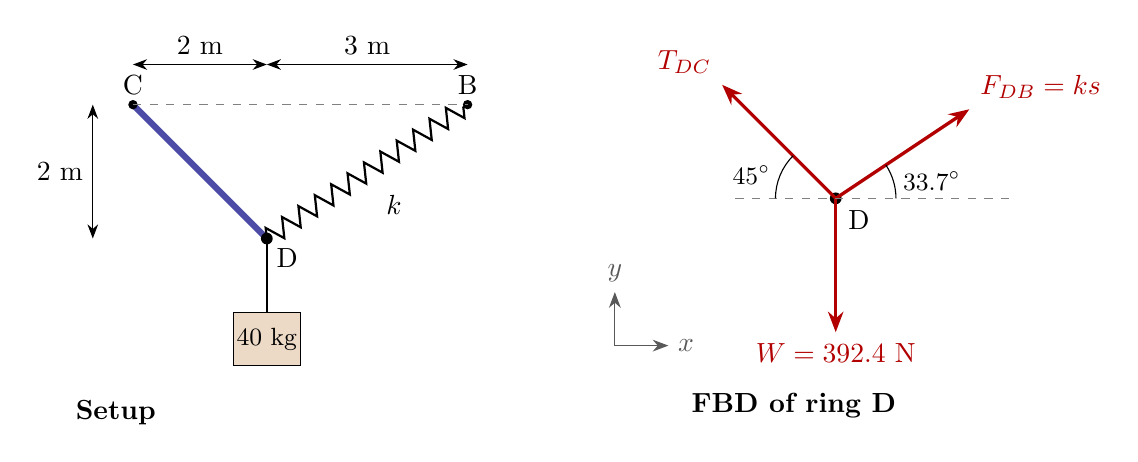
\begin{tikzpicture}[scale=0.85]
  % setup
  \draw[mem] (-2,2) -- (0,0);
  \draw[decorate,decoration={zigzag,segment length=2.5mm,amplitude=1.2mm},thick] (0,0) -- (3,2);
  \fill (-2,2) circle (2pt) node[above] {C};
  \fill (3,2) circle (2pt) node[above] {B};
  \fill (0,0) circle (2.5pt) node[below right] {D};
  \draw[thick] (0,0) -- (0,-1.1); \draw[fill=brown!30] (-0.5,-1.1) rectangle (0.5,-1.9);
  \node at (0,-1.5) {\small 40 kg};
  \draw[dashed,gray] (-2,2) -- (3,2);
  \draw[dimn] (-2,2.6) -- (0,2.6) node[midway,above] {2 m};
  \draw[dimn] (0,2.6) -- (3,2.6) node[midway,above] {3 m};
  \draw[dimn] (-2.6,2) -- (-2.6,0) node[midway,left] {2 m};
  \node at (1.9,0.5) {$k$};
  \node[anchor=west] at (-3,-2.6) {\textbf{Setup}};

  % FBD of D
  \begin{scope}[xshift=8.5cm,yshift=0.6cm]
    \fill (0,0) circle (2.5pt) node[below right=1pt] {D};
    \draw[ax] (-3.3,-2.2) -- (-2.5,-2.2) node[right] {$x$};
    \draw[ax] (-3.3,-2.2) -- (-3.3,-1.4) node[above] {$y$};
    \draw[frc] (0,0) -- ({-2.4/sqrt(2)},{2.4/sqrt(2)}) node[above left] {$T_{DC}$};
    \draw[frc] (0,0) -- ({3*2.4/sqrt(13)},{2*2.4/sqrt(13)}) node[above right] {$F_{DB}=ks$};
    \draw[frc] (0,0) -- (0,-2) node[below] {$W=392.4$ N};
    \draw[dashed,gray] (-1.5,0) -- (2.6,0);
    \draw (0.9,0) arc (0:33.7:0.9) node[midway,right] {\small $33.7^\circ$};
    \draw (-0.9,0) arc (180:135:0.9) node[midway,left] {\small $45^\circ$};
    \node[anchor=west] at (-2.3,-3.1) {\textbf{FBD of ring D}};
  \end{scope}
\end{tikzpicture}
}{
\textbf{Weight and geometry.}
\begin{align*}
W &= mg = (40\kg)(9.81\ \mathrm{m/s^2}) = 392.4\N\\
L_{DC} &=\sqrt{2^2+2^2}=\sqrt{8}\m, \qquad L_{DB}=\sqrt{3^2+2^2}=\sqrt{13}=3.606\m
\end{align*}
\textbf{Equilibrium of ring D} (the vertical cord DA carries the full weight $W$):
\begin{align*}
\sum F_x = 0:&\quad -T_{DC}\,\frac{2}{\sqrt{8}} + F_{DB}\,\frac{3}{\sqrt{13}} = 0
   \;\Rightarrow\; T_{DC} = \frac{3\sqrt{2}}{\sqrt{13}}\,F_{DB}\\
\sum F_y = 0:&\quad T_{DC}\,\frac{2}{\sqrt{8}} + F_{DB}\,\frac{2}{\sqrt{13}} - W = 0
\end{align*}
Substituting $T_{DC}\,(2/\sqrt{8}) = T_{DC}/\sqrt{2} = 3F_{DB}/\sqrt{13}$:
\[
\frac{3F_{DB}}{\sqrt{13}} + \frac{2F_{DB}}{\sqrt{13}} = W
\;\Rightarrow\; F_{DB} = \frac{\sqrt{13}}{5}\,W = \frac{3.606}{5}(392.4\N) = 283\N
\]
(and $T_{DC} = 333\N$).

\textbf{Spring law} $F_{DB}=ks$ gives the stretch, and $s = L_{DB}-\ell_0$ gives the unstretched length:
\[
s = \frac{F_{DB}}{k} = \frac{283\N}{180\ \mathrm{N/m}} = 1.57\m
\qquad\Rightarrow\qquad
\ell_0 = L_{DB} - s = 3.606\m - 1.572\m = 2.03\m
\]
}{
$\ell_0 = 2.03\m$ (spring force $F_{DB}=283\N$, stretch $s=1.57\m$).
}

% =========================================================
% PROBLEM 6
% =========================================================
\problempage{6}{
Cords BC, BD, AB, AE and AH hold a hook H at A. Cord BD has a 3-4-5 slope (4 horizontal, 3 vertical), AB makes $60^\circ$ with the horizontal, BC and AE are horizontal. Each cord carries at most 500 N. \textbf{Find} the largest mass $m$ that can hang from H.
}{
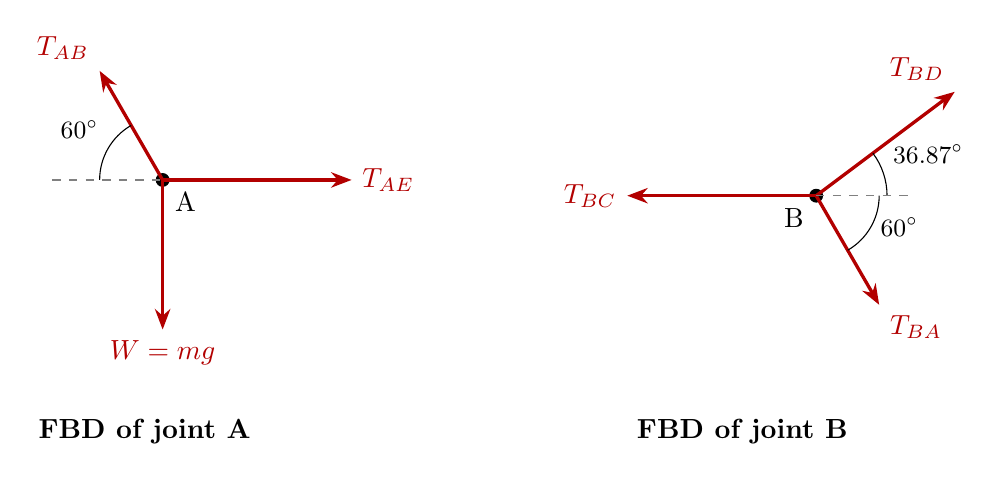
\begin{tikzpicture}[scale=1.0]
  % FBD of A
  \fill (0,0) circle (2.5pt) node[below right=1pt] {A};
  \draw[frc] (0,0) -- (2.4,0) node[right] {$T_{AE}$};
  \draw[frc] (0,0) -- ({-1.6*cos(60)},{1.6*sin(60)}) node[above left] {$T_{AB}$};
  \draw[frc] (0,0) -- (0,-1.9) node[below] {$W=mg$};
  \draw[dashed,gray] (-1.4,0) -- (0,0);
  \draw (-0.8,0) arc (180:120:0.8) node[midway,above left] {\small $60^\circ$};
  \node[anchor=west] at (-1.7,-3.2) {\textbf{FBD of joint A}};
  % FBD of B
  \begin{scope}[xshift=8.3cm,yshift=-0.2cm]
    \fill (0,0) circle (2.5pt) node[below left=1pt] {B};
    \draw[frc] (0,0) -- (-2.4,0) node[left] {$T_{BC}$};
    \draw[frc] (0,0) -- ({2.2*0.8},{2.2*0.6}) node[above left] {$T_{BD}$};
    \draw[frc] (0,0) -- ({1.6*cos(60)},{-1.6*sin(60)}) node[below right] {$T_{BA}$};
    \draw (0.9,0) arc (0:36.87:0.9) node[midway,above right] {\small $36.87^\circ$}; 
    \draw (0.8,0) arc (0:-60:0.8) node[midway,right] {\small $60^\circ$};
    \draw[dashed,gray] (0,0) -- (1.2,0);
    \node[anchor=west] at (-2.4,-3.0) {\textbf{FBD of joint B}};
  \end{scope}
\end{tikzpicture}
}{
Cord AB pulls A up and to the left, so at B the cord pulls back down and to the right ($T_{BA}=T_{AB}$). Work in terms of the weight $W = mg$, then apply the 500 N limit to the most heavily loaded cord.

\textbf{Joint A} ($T_{AH}=W$ supports the hook):
\begin{align*}
\sum F_y = 0:&\quad T_{AB}\sin60^\circ - W = 0 \;\Rightarrow\; T_{AB} = \frac{W}{\sin60^\circ} = 1.155\,W\\
\sum F_x = 0:&\quad T_{AE} - T_{AB}\cos60^\circ = 0 \;\Rightarrow\; T_{AE} = 0.577\,W
\end{align*}
\textbf{Joint B} ($T_{BA}=T_{AB}=1.155W$, direction $(\cos60^\circ,-\sin60^\circ)$; BD direction $(\tfrac45,\tfrac35)$):
\begin{align*}
\sum F_y = 0:&\quad \tfrac{3}{5}T_{BD} - T_{AB}\sin60^\circ = 0 \;\Rightarrow\; T_{BD} = \frac{W}{0.6} = 1.667\,W\\
\sum F_x = 0:&\quad \tfrac{4}{5}T_{BD} + T_{AB}\cos60^\circ - T_{BC} = 0
  \;\Rightarrow\; T_{BC} = 0.8(1.667\,W) + 0.5(1.155\,W) = 1.911\,W
\end{align*}
The largest tension coefficient is $T_{BC}=1.911\,W$:
\[
T_{BC} = 500\N \;\Rightarrow\; W = \frac{500\N}{1.911} = 261.7\N
\;\Rightarrow\; m = \frac{W}{g} = \frac{261.7\N}{9.81\ \mathrm{m/s^2}} = 26.7\kg
\]
Check the others at this load: $T_{BD}=436\N$, $T_{AB}=302\N$, $T_{AE}=151\N$, all below 500 N.
}{
$m_{\max} = 26.7\kg$ (cord BC governs, at $T_{BC}=500\N$).
}

% =========================================================
% PROBLEM 7
% =========================================================
\problempage{7}{
A 20 kg crate hangs from O, held by two springs OA and OB (each $\ell_0=2$ m, $k=300$ N/m) lying along the horizontal axes and cord OC whose end C is 6 m and 4 m horizontally and 12 m vertically from O. \textbf{Find} the stretch $s_{OA}$ and $s_{OB}$ in each spring for equilibrium.
}{
\begin{tikzpicture}[x={(-0.5cm,-0.35cm)},y={(0.7cm,0cm)},z={(0cm,0.38cm)}]
  \draw[ax] (0,0,0) -- (9,0,0) node[below left] {$x$};
  \draw[ax] (0,-6,0) -- (0,7,0) node[right] {$y$};
  \draw[ax] (0,0,0) -- (0,0,15) node[above] {$z$};
  \fill (0,0,0) circle (2pt);
  \node[above right=1pt] at (0,0,0) {O};
  \draw[frc] (0,0,0) -- (-5,0,0) node[above right] {$F_B$};
  \draw[frc] (0,0,0) -- (0,-5,0) node[above left] {$F_A$};
  \draw[frc] (0,0,0) -- (0.6,1.0,6.5) node[right] {$T_{OC}$};
  \draw[frc] (0,0,0) -- (0,0,-11) node[below] {$W=196.2$ N};
  \node[anchor=west,align=left,font=\small] at (2.4,2.6) {$\vec r_{OC}=(6,\,4,\,12)$ m\\ (C is 6 m along $x$,\\ 4 m along $y$, 12 m up)};
\end{tikzpicture}
\\[2pt]\small FBD of O: $F_A$ pulls toward A (along $-y$), $F_B$ toward B (along $-x$); $\vec r_{OC}=(6,4,12)$ m.
}{
\textbf{Weight and cord direction.}
\begin{align*}
W &= (20\kg)(9.81\ \mathrm{m/s^2}) = 196.2\N\\
\vec{r}_{OC} &= (6\,\hat{\imath}+4\,\hat{\jmath}+12\,\hat{k})\m, \qquad |\vec{r}_{OC}|=\sqrt{36+16+144}=14\m
\end{align*}
\[
\vec{T}_{OC} = T_{OC}\,\frac{6\,\hat{\imath}+4\,\hat{\jmath}+12\,\hat{k}}{14},\qquad
\vec{F}_B = -F_B\,\hat{\imath},\qquad \vec{F}_A = -F_A\,\hat{\jmath},\qquad \vec{W} = -196.2\,\hat{k}\N
\]
\textbf{Equilibrium of O}, $\sum\vec F = \vec 0$:
\begin{align*}
\sum F_z = 0:&\quad \tfrac{12}{14}T_{OC} - 196.2\N = 0 \;\Rightarrow\; T_{OC} = 228.9\N\\
\sum F_x = 0:&\quad \tfrac{6}{14}T_{OC} - F_B = 0 \;\Rightarrow\; F_B = \tfrac{6}{14}(228.9\N) = 98.1\N\\
\sum F_y = 0:&\quad \tfrac{4}{14}T_{OC} - F_A = 0 \;\Rightarrow\; F_A = \tfrac{4}{14}(228.9\N) = 65.4\N
\end{align*}
\textbf{Spring law} $F=ks$ (the unstretched length $\ell_0=2$ m is not needed for the stretch):
\[
s_{OA} = \frac{F_A}{k} = \frac{65.4\N}{300\ \mathrm{N/m}} = 0.218\m,\qquad
s_{OB} = \frac{F_B}{k} = \frac{98.1\N}{300\ \mathrm{N/m}} = 0.327\m
\]
}{
$s_{OA} = 0.218\m$ and $s_{OB} = 0.327\m$ (spring forces $65.4\N$ and $98.1\N$; cord tension $T_{OC}=229\N$).
}

% =========================================================
% PROBLEM 8
% =========================================================
\problempage{8}{
An 800 lb cylinder hangs from ring A, supported by chains AB, AC and AD attached to a horizontal circle of radius 1 ft (in the $z=0$ plane), with $d=1$ ft below it. C is on the $+x$ axis, D on the $-y$ axis, and B lies $135^\circ$ from each of them. \textbf{Find} the tension in each chain.
}{
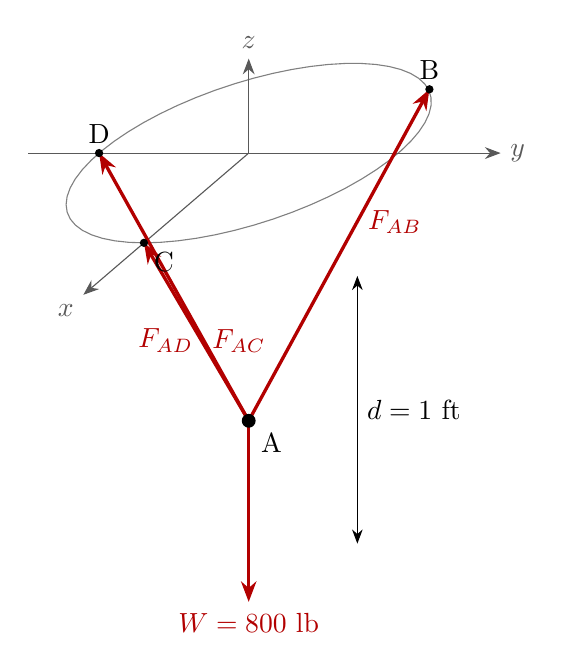
\begin{tikzpicture}[x={(-0.7cm,-0.6cm)},y={(1cm,0cm)},z={(0cm,1cm)}]
  % top view circle and points
  \draw[thin,gray] plot[domain=0:360,samples=60] ({cos(\x)*1.9},{sin(\x)*1.9},3.4);
  \coordinate (A) at (0,0,0);
  \coordinate (B) at (-1.35,1.35,3.4);
  \coordinate (C) at (1.9,0,3.4);
  \coordinate (D) at (0,-1.9,3.4);
  \draw[ax] (0,0,3.4) -- (3.0,0,3.4) node[below left] {$x$};
  \draw[ax] (0,-2.8,3.4) -- (0,3.2,3.4) node[right] {$y$};
  \draw[ax] (0,0,3.4) -- (0,0,4.6) node[above] {$z$};
  \draw[frc] (A) -- (B) node[pos=0.6,right] {$F_{AB}$};
  \draw[frc] (A) -- (C) node[pos=0.45,right] {$F_{AC}$};
  \draw[frc] (A) -- (D) node[pos=0.3,left] {$F_{AD}$};
  \draw[frc] (A) -- (0,0,-2.3) node[below] {$W=800$ lb};
  \fill (A) circle (2.5pt) node[below right=1pt] {A};
  \fill (B) circle (1.5pt) node[above] {B};
  \fill (C) circle (1.5pt) node[below right] {C};
  \fill (D) circle (1.5pt) node[above] {D};
  \draw[dimn] (2.6,3.2,3.4) -- (2.6,3.2,0);
  \node[right] at (2.6,3.2,1.7) {$d=1$ ft};
\end{tikzpicture}
\\[2pt]\small FBD of ring A (all three chains pull A up toward B, C, D). Points: A$(0,0,-1)$, B$(-0.707,0.707,0)$, C$(1,0,0)$, D$(0,-1,0)$ ft.
}{
\textbf{Chain vectors from A} (A at $(0,0,-1)$ ft; the anchors lie on the unit circle, with B at $135^\circ$ from both C and D):
\begin{align*}
\vec r_{AB} &= (-0.707,\;0.707,\;1)\ft, & |\vec r_{AB}| &= \sqrt{0.5+0.5+1}=1.414\ft\\
\vec r_{AC} &= (1,\;0,\;1)\ft, & |\vec r_{AC}| &= 1.414\ft\\
\vec r_{AD} &= (0,\;-1,\;1)\ft, & |\vec r_{AD}| &= 1.414\ft
\end{align*}
\textbf{Force vectors} ($\vec F=F\,\vec r/|\vec r|$), plus the weight $\vec W=-800\,\hat k\lb$:
\begin{align*}
\vec F_{AB} &= F_{AB}\,(-0.5\,\hat\imath + 0.5\,\hat\jmath + 0.707\,\hat k), \\
\vec F_{AC} &= F_{AC}\,(0.707\,\hat\imath + 0.707\,\hat k), \qquad
\vec F_{AD} = F_{AD}\,(-0.707\,\hat\jmath + 0.707\,\hat k)
\end{align*}
\textbf{Equilibrium of A}, $\sum\vec F=\vec 0$:
\begin{align*}
\sum F_x = 0:&\quad -0.5\,F_{AB} + 0.707\,F_{AC} = 0 \;\Rightarrow\; F_{AC} = 0.707\,F_{AB}\\
\sum F_y = 0:&\quad 0.5\,F_{AB} - 0.707\,F_{AD} = 0 \;\Rightarrow\; F_{AD} = 0.707\,F_{AB}\\
\sum F_z = 0:&\quad 0.707\,(F_{AB}+F_{AC}+F_{AD}) - 800\lb = 0
\end{align*}
Substituting the first two into the third: $0.707\,F_{AB}(1+0.707+0.707) = 800\lb \Rightarrow 1.707\,F_{AB} = 800\lb$, so
\[
F_{AB} = \frac{800\lb}{1.707} = 469\lb,\qquad
F_{AC} = F_{AD} = 0.707\,(468.6\lb) = 331\lb
\]
Check: $0.707(469+331+331)\lb = 800\lb$ \checkmark
}{
$F_{AB} = 469\lb$, $F_{AC} = 331\lb$, $F_{AD} = 331\lb$.
}

\end{document}